\documentclass[11pt,
compress,
%% handout, 
%% dvips,
%% trans
]{beamer}
%% Try the class options [notes], [notes=only], [trans], [handout],
%% [red], [compress], [draft], [class=article] and see what happens!

\usepackage{bm}
\usepackage{booktabs}
\usepackage[scale=2]{ccicons}
%\usepackage{minted}
\usepackage{amsmath,amsthm,amssymb,amsfonts}
\newcommand*{\TakeFourierOrnament}[1]{{%
		\fontencoding{U}\fontfamily{futs}\selectfont\char#1}}
\newcommand*{\danger}{\TakeFourierOrnament{66}}
\usepackage[export]{adjustbox}
%\usepgfplotslibrary{dateplot}
\usepackage{wrapfig}
\usepackage{ragged2e}
\usepackage{xcolor}
\newcommand{\red}{\color{red}}
\newcommand{\mb}{\color{blue}}
\newcommand{\blue}{\color{blue}}
\newcommand{\orange}{\color{orange}}
\newcommand{\green}{\color{green}}
\usepackage{multirow}
\usepackage{tabularx}
\usepackage{transparent}
\usepackage{graphicx}
\usepackage{caption}
\newcommand{\mnb}{\color{violet}}
\newcommand{\emer}{\color{Emerald}}
\newcommand{\fogr}{\color{ForestGreen}}
\newcommand{\redor}{\color{RedOrange}}
\newcommand{\ceru}{\color{Cerulean}}
\newcommand{\yelor}{\color{black}}
\newcommand{\ored}{\color{olive}}

\newcommand{\ubar}[1]{\text{\b{$#1$}}}

\usepackage{caption}
\usepackage{subcaption}
%\lstset{language=R,
	%	basicstyle=\scriptsize\ttfamily,
	%	stringstyle=\color{black},
	%	otherkeywords={0,1,2,3,4,5,6,7,8,9},
	%	morekeywords={TRUE,FALSE},
	%	deletekeywords={data,frame,length,as,character},
	%	keywordstyle=\color{black},
	%	commentstyle=\color{blue},
	%	escapechar={?}, 
	%}
\usepackage[utf8]{inputenc}
\usepackage[english]{babel}
\usepackage{hyperref}
\usepackage{amsmath,amsthm,amssymb,pgf}
\usepackage{comment,multicol}
%\usepackage{color}
\usepackage{rotating, listings}
\usepackage{tikz}
\usepackage{booktabs}

%% If we deo not want e``(a) Text'' but ``Text'' in subfigures.
%\usepackage{subfigure}
%\renewcommand{\thesubfigure}{\null}

%% Set custom font (Source Sans Pro)


%%\usetheme{Madrid}
\usetheme{CambridgeUS}
%%\usecolortheme{default}
\usecolortheme{dolphin}


%% KAUST saturated shades
%% Purple , R 109 G 36 B 99 , HEX# 6D2463
\definecolor{kaustpurplesaturatedshade}{RGB}{109,36,99}
%% Blue , R 0 G 59 B 117 , HEX# 003B75
\definecolor{kaustbluesaturatedshade}{RGB}{0,59,117}
%% Turquoises , R 0 G 76 B 89 , HEX# 004C59
\definecolor{kaustturquoisessaturatedshade}{RGB}{0,76,89}
%% Greens , R 89 G 84 B 3 , HEX# 595403
\definecolor{kaustgreenssaturatedshade}{RGB}{89,84,3}
%% Yellow , R 100 G 60 B 0 , HEX# 643C00
\definecolor{kaustyellowsaturatedshade}{RGB}{100,60,0}
%% Orange , R 128 G 73 B 0 , HEX# 804900
\definecolor{kaustorangesaturatedshade}{RGB}{128,73,0}

%% KAUST Gray , R 181 G 171 B 161 , HEX# B5ABA1
\definecolor{kaustgrayfullcolor}{RGB}{181,171,161}

%% User custom KAUST color scheme
\setbeamercolor*{structure}{bg=kaustgrayfullcolor!20,fg=kaustbluesaturatedshade}
%% \setbeamercolor*{palette primary}{use=structure,fg=white,bg=structure.fg}
%% \setbeamercolor*{palette primary}{use=structure,fg=white,bg=structure.fg}
%% \setbeamercolor*{palette secondary}{use=structure,fg=white,bg=structure.fg!75}
%% \setbeamercolor*{palette tertiary}{use=structure,fg=white,bg=structure.fg!50!black}
%% \setbeamercolor*{palette quaternary}{fg=white,bg=black}
%% \setbeamercolor{section in toc}{fg=black,bg=white}
%% \setbeamercolor{alerted text}{use=structure,fg=structure.fg!50!black!80!black}
%% \setbeamercolor{titlelike}{parent=palette primary,fg=structure.fg!50!black}
%% \setbeamercolor{frametitle}{bg=gray!10!white,fg=PineGreen}
%% \setbeamercolor*{titlelike}{parent=palette primary}


%% %% set logo, default position bottom right corner
%% \logo{\includegraphics[height=0.75cm]{./figures/KAUST-logo-seed.pdf}}
%% add logo to frame title, position using tikz
\addtobeamertemplate{frametitle}{}{%
    \begin{tikzpicture}[remember picture,overlay]
        \node[anchor=north east,yshift=-9pt] at (current page.north
        east)%%
        {
\includegraphics[height=0.75cm]{./up_logo.png}};
    \end{tikzpicture}
}
\usepackage{verbatim}
\setbeamercovered{transparent=15}

\usepackage{algorithm}
\usepackage{algorithmic}

\newcommand{\W}{\mathcal{W}}
\newcommand{\E}{\mathcal{E}}

\def\Prob{\text{Prob}}
\def\E{\text{E}}
\def\Cov{\text{Cov}}
\def\Corr{\text{Corr}}
\def\Var{\text{Var}}
\def\Prec{\text{Prec}}

\def\qedbox{\ifvmode\else\unskip\fi~\penalty10000 \hfill{\large$\blacksquare$}}
\def\Fig#1{Figure~\ref{#1}}
\def\Tab#1{Table~\ref{#1}}
\def\Sec#1{Section~\ref{#1}}
\def\Thm#1{Theorem~\ref{#1}}
\def\Def#1{Definition~\ref{#1}}
\def\Lem#1{Lemma~\ref{#1}}
\def\Alg#1{Algorithm~\ref{#1}}
\def\Ex#1{Example~\ref{#1}}
\def\Cor#1{Corollary~\ref{#1}}
\def\eref#1{(\ref{#1})}
\def\miscinfo#1#2{{\footnotesize\indent\textsc{#1: }\ignorespaces #2}}
\def\R{\mathbb{R}}
\def\mm#1{\ensuremath{\boldsymbol{#1}}} %% version: amsmath
\def\mv#1{\ensuremath{\boldsymbol{#1}}} %% version: amsmath
\def\logit{\text{logit}}


\title[Spatial survival]{
    Spatial survival and joint models with INLA}

\author[Janet van Niekerk]{Janet van Niekerk\\
	\tiny{Janet.vanNiekerk@up.ac.za\\
University of Pretoria, South Africa\\
\vspace{2cm}}
   }

\date[June 2026]{}

\usepackage{listings}
\lstset{language=C}
\let\MyIncludeSourceFontSize\footnotesize
\let\MyIncludeFontSize\small
\def\MyIncludeSource#1{\lstset{basicstyle=\MyIncludeSourceFontSize}\lstinputlisting{#1}%%
    \lstset{basicstyle=\MyIncludeFontSize}}

\begin{document}

{
  \usebackgroundtemplate{\texttransparent{0.5}{
\includegraphics[width=1.05\paperwidth]{./up_building3.png}}}
  \begin{frame}
    \titlepage
  \end{frame}
}

\begin{frame}
\frametitle{Outline}
\tableofcontents
\end{frame}

\section{Introduction}

\begin{frame}
	\frametitle{Joint Model}
	\vspace{-0.8cm}

	A joint model simultaneously models longitudinal (time-dependent) data and Time-To-Event (TTE) data whilst accounting for censoring.\\ \ \\

	Consider an example of cancer patients undergoing a specific treatment. In this case, the longitudinal data could be the size of a tumor and the event of interest could be whether the patient dies under that treatment. 
\end{frame}


\begin{frame}
	\frametitle{Longitudinal Model}
	\vspace{-0,8cm}

	A longitudinal model, say $m(t, \ubar{\Psi}_i)$, allows us to model a variable of interest (often referred to as the biomarker) as time progresses. \\ \ \\

	In our example, modeling how a patients tumor changes in size allows predictions to be made regarding patient outcomes so that necessary decisions can be made in time. \\ \ \\

	Different patients will, of course, exhibit differences in how their tumors progress and how they respond to any treatments. Thus, the longitudinal model is typically a \bm{{\mb mixed-effect model}}, utilizing the fixed and random effects of patient $i$ ($\ubar{\Psi}_i$) to account for within-patient correlation and allowing for the modeling of multiple patients.

\end{frame}


\begin{frame}
	\frametitle{Survival Model}
	\vspace{-0.8cm}

	TTE data is modeled through a survival model. This is done by determining the relevant \bm{{\mb hazard function}} $h_i(t)$, defined as the risk of a patient experiencing the event of interest at a specific time. i.e. 

$$
h_i(t) = \lim_{\Delta t \to 0} \frac{\mathrm{P}(t < T_i \le t + \Delta t \mid T_i > t)}{\Delta t}
$$

	It is within the survival model that censoring is accounted for. Censoring is defined as the case where the Time-To-Event is not observed in a patient for any reason. For example, a patient may no longer be able to participate in the study after moving or the event may simply have not occurred during the study period. \bm{{\mb In survival models, censoring is assumed random.}}
\end{frame}


\begin{frame}
	\frametitle{Why a Joint Model?}
	\vspace{-0.8cm}

	We expect that a patient with a large tumor to have a lower survivability. Additionally, once those with low survivability die, we expect that the remaining patients to have smaller tumors. Thus, \bm{{\mb the longitudinal model and survival model both effect each other and are not independent}}. Therefore, \bm{{\mb a joint model}} that models both processes and their dependence on each other \bm{{\mb jointly}} is required.\\ \ \\

	This allows joint models to account non-random censoring. For example, a patient may see that their tumor is worsening under the study and decide to pull out to seek another treatment.\\ \ \\

	Ultimately, by making use of a joint model, one can create a more accurate model than by modeling either process alone, allowing for more accurate conclusions about the efficacy of the treatment being studied.
\end{frame}


\begin{frame}
	\frametitle{Non-Linearity}
	\vspace{-0.8cm}

	A typical, linear joint model may be:

$$
h_i(t, \ubar{ \Psi }_i) = h_0(t) \cdot e^{\beta \cdot f(t, \ubar{\Psi}_i) + \gamma \cdot g(\ubar{\Psi}_i)}
$$

where $h_0$ is the baseline hazard function, $f(t, \ubar{\Psi}_i)$ is the indirect effects and is some function of $m(t, \ubar{\Psi}_i)$, and $g(\ubar{\Psi}_i)$ is the direct effects.\\ \ \\

However, say that instead of simply $\beta \cdot  f(t, \ubar{\Psi}_i)$, we had some non-linear function of $f$, such as a square root function, a spline, or a log function. This would be a non-linear joint model.
\end{frame}

\begin{frame}
	\frametitle{Why a Non-Linear Joint model?}
	\vspace{-0.8cm}

\begin{wrapfigure}{r}{0.5\textwidth}
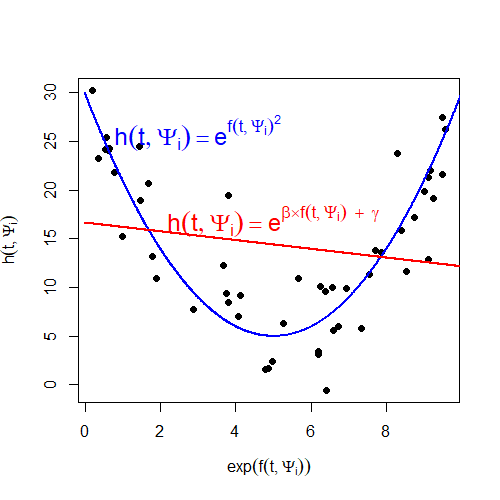
\includegraphics[width=0.5\textwidth, right]{simexample}
\end{wrapfigure}
Consider the case of type I\\ diabetes patients. These patients are at greater risk of very high and very low blood glucose levels which can both cause seizures. \\ \ \\


You can see in the figure, a simulated example of this scenario, where the non-linear model performs very well while the linear model fails to conclude significance with a p-value of $0.23$.
\end{frame}

\section{Survival analysis}

\begin{frame}
	\huge Survival analysis
\end{frame}


\begin{frame}[fragile]
	\frametitle{Time to event}
	\vspace{-0.8cm}
	What about the \bm{{\mb number of events}}? \\ \ \\
	
	What about the \bm{{\mb time elapsed}} between the beginning of the trial and the event? \\ \ \\
	
	\centering
	%\vspace{-0.5cm} \includegraphics[scale=0.4]{surv5.png}
	
\end{frame}





\begin{frame}[fragile]
	\frametitle{Random censoring / informative censoring}
	\vspace{-0.8cm}
	
	\begin{itemize}
		\item \bm{{\mb Random (or non-informative)}} censoring: Patients are censored due to reasons unrelated to the study.
	\end{itemize}
	\small
	Examples: The event has not occurred at the end of the follow-up; Patient moves to another country and cannot continue its participation to the trial.
	\normalsize
	\pause
	
	\begin{itemize}
		\item \bm{{\mb Informative censoring}}: Patients are censored due to reasons related to the study.
	\end{itemize}
	\small
	Examples: Patient decides to stop taking the treatment because of side effects; Patient is too sick and clinicians decide to switch to another treatment\textit{ (assuming independent censoring in this case would lead to underestimation of the hazard)};\\
	Patient feels cured by an effective treatment and may no longer feel the need to follow-up \textit{(assuming independent censoring in this case would lead to overestimation of the hazard)}.\\
	
	\textbf{In survival analysis, we usually need to assume censoring is random!}
	
\end{frame}

\begin{frame}[fragile]
	\frametitle{Survival data - Survival analysis}
	\vspace{-0.8cm}
	
	\bm{{\mb Survival analysis}} is used to analyze data in which \bm{{\mb the time
			until the event is of interest}}. The response is often referred to
	as a failure time, survival time, or event time.\\
	
	
	\centering
	%\includegraphics[scale=0.3]{surv6.png}
	
	\raggedright
	=> Not easy to compare! 
	
	Moreover clinical trials usually include hundreds of patients.
\end{frame}

\begin{frame}[fragile]
	\frametitle{Quantities of interest in survival analysis}
	\vspace{-0.9cm}
	Let \bm{{\mb $T$}} denote the positive continuous response variable that represents the \bm{{\mb elapsed time between the beginning of the follow-up and the event of interest}}. There are many ways to represent and describe the distribution of $T$.\\
	
	\begin{itemize}
		\item \bm{{\mb Hazard function:}} Instantaneous \bm{{\mb risk of event.}} $$\lambda(t)=\lim\limits_{h \rightarrow 0^+} \frac{P(t\leq T < t+h | T>t)}{h}$$
		
		\item \bm{{\mb Survival function:}} Probability of being alive up to time $t$ (i.e., dying after $t$). $$S(t)=P(T>t)=\exp(-\int_{0}^{t} \lambda(u)du)$$
	\end{itemize}
	
\end{frame}




\begin{frame}[fragile]
	\frametitle{Parametric baseline}
	\vspace{-1cm}
	
	$$\lambda_i(t)=\lambda_{0}(t)\ \textrm{exp}\left(\beta_{drug} * drug_i + \beta_{x} * x_i\right)$$
	\mb{Exponential} -  $\lambda_{0}(t) = \lambda_{0}$ (constant risk)\\ 
	
	\mb{Weibull} - $\lambda_{0}(t) = \alpha t ^{\alpha - 1}$\\
	\begin{itemize}
		\item \textbf{ $\alpha> 1$:} Hazard increases the longer you survive (Type I)
		\item \textbf{$\alpha = 1$:} Special case, exponential (Type II)
		\item \textbf{$\alpha< 1$:} Hazard decreases the longer you survive (Type III)
	\end{itemize}

%\includegraphics[scale=0.2]{survivorship.png}\\
	
\end{frame}

\section{Time-dependent covariates in survival models}

\begin{frame}
	
	\huge Time-dependent covariates in survival models
\end{frame}

\begin{frame}[fragile]
	\frametitle{Time-dependent covariates}
	\vspace{-1cm}
	It is possible to include \bm{{\mb time-dependent covariates}} in a survival model, they can be classified into
	two categories:
	\begin{itemize}
		\item \bm{{\mb Exogeneous}} (or external) covariates remain measurable and their distribution is unchanged
		after the occurrence of the event.
		\item \bm{{\mb Endogeneous}} (or internal) covariates’ distribution is affected by the event.
	\end{itemize}
	The proportional hazards model can handle exogeneous time-dependent covariates but the likelihood requires \bm{{\mb knowing the value of these covariates for all subjects at risk for each event time}}.
\end{frame}

\begin{frame}[fragile]
	\frametitle{Time-dependent covariates }
	\vspace{-1cm}
	When covariates measurements does not coincide with event times in the sample, \bm{{\mb models are required to impute values}} at the times of events.
	
	Likelihood = $\prod_{i=1}^{N} S_i(t)\lambda_i(t)^{[Event indicator]}$\\
	where $S(t)=\exp(-\int_{0}^{t} \lambda(u)du)$ and $\lambda_i(t)=\lambda_{0}(t)\ \textrm{exp}\left(X_i(t) \ \bm \gamma \right)$\\
	
	However, most biomarkers of interest in clinical research are endogeneous variables, their \bm{{\mb values are affected}} by a \bm{{\mb change in the risk}} of occurrence of the event.\\
	
	\small
	For example in a cancer clinical trial, if a \bm{{\mb treatment reduces}} both the \bm{{\mb risk of death}} and the \bm{{\mb size of tumors}}, adjusting a survival model on the tumors size may severely \bm{{\mb bias the effect of treatment}} on the risk of death.
\end{frame}
\begin{frame}[fragile]
\frametitle{Idea?}
\vspace{-0.7cm}

Can we have a \bm{{\mb statistical model}} that evaluates \bm{{\mb simultaneously}} the effect of treatment on the tumors size and the risk of death?\\

Useful because when death occurs => no more measurements of tumors size!\\
Maybe we never observe big tumors because a patient with big tumors die (\bm{{\mb informative censoring}}).\\

The risk of death for a patient with big tumor is higher compared to a patient with small tumors (\bm{{\mb recorded heterogeneity of the population}}).

\end{frame}

\section{Joint models}

\begin{frame}
	\huge Joint models
\end{frame}



\begin{frame}[fragile]
	\frametitle{Joint modeling - underlying idea}
	\vspace{-0.7cm}
	
	Joint modeling consists in \bm{{\mb simultaneously}} modeling \bm{{\mb multiple outcomes}} while taking into account their \bm{{\mb association}}. The outcomes are either \bm{{\mb longitudinal}} or \bm{{\mb time to an event}} of interest (e.g., death in health research). \\
	
	Joint models are popular in health research because it is common to observe \bm{{\mb longitudinal markers censored by a terminal event}} with interest in the analysis of the longitudinal marker trajectory and the risk of the terminal event as well as their relationship.\\
	
\end{frame}


\begin{frame}[fragile]
	\frametitle{Joint modeling - Examples}
	\vspace{-0.7cm}
	A few examples of recent applications of joint models:
	\begin{itemize}
		\item Cancer tumor dynamics and the risk of death
		\item Analysis of CD4 lymphocytes counts and AIDS survival
		\item Prostate-specific antigen dynamics and the risk of cancer recurrence
		\item Dynamics of aortic gradient and aortic regurgitations and their relationship with the competing risks of death or reoperation in the field of cardiac surgery
		\item Cognitive markers’s relationship with the time to onset of Alzheimer’s disease
		\item Jointly modeling forest fires ignition, number of fires and the proportion of burned area in mainland Portugal aggregated by years and regions
	\end{itemize}
\end{frame}

\begin{frame}[fragile]
	\frametitle{Joint modeling Longitudinal and Survival data}
	\vspace{-0.7cm}
	\begin{itemize}
		\item Can \bm{{\mb efficiently utilize all available information}} to limit costs and optimize outcomes.\pause
		\item Dynamic risk predictions for personalized care.\pause
		\item Have interesting properties for \bm{{\mb mediation analysis}} (decomposition of a treatment effect into \bm{{\mb direct and indirect effects}} (could be a promising tool in the shift toward causality in clinical trials evaluation, see ICH E9 addendum recommendations).\pause
		\item Evaluation of \bm{{\mb surrogate markers}}.
	\end{itemize}
	
	
	\centering
	%\visible<3, 4>{\includegraphics[scale=0.27]{./JMStructure.png}}
	
\end{frame}

\begin{frame}[fragile]
	\frametitle{Association Structures}
	\vspace{-0.8cm}
	\small
	\centering
	\begin{tabularx}{\textwidth}{|>{\RaggedRight}p{3cm}|>{\RaggedRight}p{3.0cm}|>{\RaggedRight}X|}
		\hline
		\textbf{Association} & \textbf{Shared Component} & \textbf{Key Question} \\
		\hline
		\textbf{Shared Random Effects (SRE)} & Random Intercept/Slope ($b_{i0}, b_{i1}$) & Does an \bm{{\mb individual's underlying trajectory}} (higher baseline, faster progression) affect their risk? \\
		\hline
		\textbf{Current Value (CV)} & Full Linear Predictor ($\eta_i(t)$) & Does the \bm{{\mb current ``true'' value}} of the marker at time $t$ affect risk at time $t$? \\
		\hline
		\textbf{Current Slope (CS)} & Derivative of Linear Predictor ($\frac{d\eta_i(t)}{dt}$) & Does the current \bm{{\mb rate of change}} of the marker affect risk? \\
		\hline
		\textbf{Cumulative Value (AUC)} & Integral of Linear Predictor ($\int \eta_i(s)ds$) & Does the \bm{{\mb cumulative exposure}} to the marker over time affect risk? \\
		\hline
	\end{tabularx}
\end{frame}


\subsection{Computational approaches for inference}
\begin{frame}
	\frametitle{Software packages in R}
	Maximum likelihood - \textit{JM, joineRML, frailtypack, }\\
	Bayesian inference - MCMC-based \textit{JMbayes2}
\end{frame}

\begin{frame}[fragile]
	\frametitle{Lack of efficient algorithms!}
	\vspace{-1cm}
	
	For frequentist inference the multiple random effects included in joint models needs to be integrated out in the likelihood => \bm{{\mb multidimensional integral}} that requires numerical approximation.\\
	
	\pause
	\bm{{\mb Iterative algorithms}} (e.g., Newton-like, Monte-Carlo) have \bm{{\mb slow convergence properties}}, joint modeling has been \bm{{\mb limited}} so far by the available inference techniques and associated statistical software.
	\vfill
	\scriptsize
	{\color{purple}  Hickey, G. L., Philipson, P., Jorgensen, A., Kolamunnage-Dona, R. \textit{Joint modelling of time-to-event and multivariate longitudinal outcomes: recent developments and issues.} BMC medical research methodology, 16(1), 1-15. (2016)}
\end{frame}


\section{INLA}

\begin{frame}
	\huge INLA
\end{frame}


\begin{frame}
	\frametitle{Integrated Nested Laplace Approximations (INLA)}
	\vspace{-1cm}
	INLA is a \bm{{\mb deterministic alternative}} to the Markov chain Monte Carlo sampling methods for Bayesian inference of latent Gaussian models. \\ 
	
	\pause
	$\rightarrow$ Approximate Bayesian inference \bm{{\mb without sampling}}.\\ 
	
	\pause
	A latent Gaussian model is where the data $\pmb{Y}_i$ depends on the latent field $\pmb{\chi}$
	only through the linear predictor $\eta_i$
	and the latent field has a \bm{{\mb Gaussian distribution}} (with sparse precision).
	
	\begin{equation*}
		\pi(\pmb{\chi},\pmb{\theta})\varpropto \pi(\pmb{y}|\pmb{\chi,\theta})\pi(\pmb{\chi}|\pmb{\theta})\pi(\pmb{\theta})
	\end{equation*}
	\normalsize
	\\
	
	\pause
	Likelihood (any distribution), latent field (Gaussian), prior (any distribution).
\end{frame}


\begin{frame}
	\frametitle{Integrated Nested Laplace Approximations (INLA)}
	\vspace{-1cm}
	Many models fit with the LGM framework and thus can be fitted with INLA:\\
	\begin{itemize}
		\pause
		\item \bm{{\mb Survival models}} (AFT, Cox models, competing risks, multi-state, cure models, frailty, censoring and truncation, parametric and nonparametric hazards)
		\pause
		\item \bm{{\mb Longitudinal models}} (GLMM, zero-inflated models, proportional odds, ...)\pause
		\item \bm{{\mb Spatial and spatio-temporal models}} (CAR, ICAR, MCAR, Matern, SPDE)\pause
		\item \bm{{\mb Joint models that include multiple longitudinal and survival outcomes}}\pause
		\item and many more...
	\end{itemize}
	\vspace{0.5cm}\pause
	With a few exceptions (e.g., PK/PD models using ODE or SDE without analytical solution).
	
\end{frame}


\begin{frame} 
	\frametitle{Integrated Nested Laplace Approximations (INLA)}
	This \bm{{\mb computationally efficient}} and \bm{{\mb accurate}} algorithm is implemented in the freely available open-source R package \textit{INLA}.\\
	
	\color{purple}
	\begin{center}
		R-INLA project (\url{www.r-inla.org})
	\end{center}
	\vfill
	
	\scriptsize
	{\color{purple}  Rue, Håvard, Sara Martino, and Nicolas Chopin. \textit{Approximate Bayesian inference for latent Gaussian models by using integrated nested Laplace approximations.} Journal of the royal statistical society: Series b (statistical methodology) 71.2 (2009): 319-392.\\
		Van Niekerk, Janet, Elias Krainski, Denis Rustand, and Håvard Rue. "A new avenue for Bayesian inference with INLA." Computational Statistics \& Data Analysis 181 (2023): 1-14}
	
\end{frame}


\begin{frame}[fragile]
	\frametitle{Comparison with MLE, STAN and JMbayes2}
	\vspace{-1cm}
	\small
	\textbf{Comparison with Levenberg-Marquardt algorithm (Newton-like algorithm):}\\
	{\color{purple}  Rustand D, van Niekerk J, Rue H, Tournigand C, Rondeau V, Briollais L. \textit{Bayesian estimation of two‐part joint models for a longitudinal semicontinuous biomarker and a terminal event with INLA: Interests for cancer clinical trial evaluation.} Biometrical Journal. 2023 Apr;65(4):2100322.}\\ \ \\
	
	\textbf{Comparison with MCMC and MCEM:}\\
	{\color{purple}  Rustand, D., van Niekerk, J., Krainski, E. T., Rue, H., Proust-Lima, C. \textit{Fast and flexible inference for joint models of multivariate longitudinal and survival data using integrated nested Laplace approximations}, Biostatistics, 2023 Aug; kxad019, https://doi.org/10.1093/biostatistics/kxad019.}\\
\end{frame}

\begin{frame}[fragile]
	\frametitle{Computational Advantage of INLA}
	\vspace{-1cm}
	\begin{table}[h!]
		\centering
		\caption*{Computation Time Comparison (in seconds)}
		\label{tab:computation_time}
		\begin{tabularx}{\textwidth}{|l|X|X|X|X|}
			\hline
			\textbf{Model} & \textbf{INLA} & \textbf{MCMC (JAGS)} & \textbf{HMC (Stan)}\\
			\hline
			Proportional Hazards & 0.6 & 15 & 67\\
			\hline
			Multi-state & 0.8 & 155 & 94\\
			\hline
			Joint Model & 12 & 1754 & 949\\
			\hline
			Multivariate Joint Model & 23 & 7105 & 9426\\
			\hline
		\end{tabularx}
	\end{table}
	\begin{minipage}[t]{\textwidth}
		\linespread{0.8}\selectfont
		\footnotesize {\color{purple}  Danilo Alvares, Janet van Niekerk, Elias T. Krainski, H\aa vard Rue, Denis Rustand. \textit{Bayesian survival analysis with INLA.} Statistics in Medicine. 2024; 43(20): 3975-4010. doi: 10.1002/sim.10160}
	\end{minipage}
\end{frame}

\begin{frame}[fragile]
	\frametitle{Computation time - scaling}
	%\begin{figure}
	%	\centering
	%	\vspace{-1.0cm}
	%	\includegraphics[width=1\textwidth]{CT_scale.pdf}
	%\end{figure}
\end{frame}


\subsection{INLAjoint - user interface for survival and joint models}
\begin{frame}[fragile]
	\vspace{-0.7cm}
	\frametitle{R package: INLAjoint}
	We recently developed a \bm{{\mb flexible}} and \bm{{\mb user-friendly}} interface to fit models for survival and/or longitudinal data with INLA. The \bm{{\mb INLAjoint}} package allows to build various models with a lot of flexibility, using its main function \bm{{\mb \textit{joint()}}}:
	\begin{itemize}
		\item Univariate and multivariate \bm{{\mb survival}} outcomes (i.e., frailty models, competing risks, multi-state) fitted with \bm{{\mb proportional hazards models}}
		\item Univariate and multivariate \bm{{\mb longitudinal}} outcomes fitted with \bm{{\mb mixed effects models}}
		\item Multivariate longitudinal and survival outcomes
	\end{itemize}

	\vfill
	\footnotesize {\color{purple}  \textit{Rustand, D., Teixeira Krainski, E., Rue, H., van Niekerk, J. \textit{INLAjoint: Multivariate joint modeling for longitudinal and time-to-event outcomes with INLA.} https://github.com/DenisRustand/INLAjoint}}
\end{frame}


\section{Spatial models}

\begin{frame}
	$$\lambda_i(t)=\lambda_{0}(t)\ \textrm{exp}\left(\pmb\beta \pmb x + \pmb f\right)$$
	$f$ are random effects that can facilitate components indexed by \mb{space}, time, groups, clusters...
\end{frame}
\begin{frame}
	\frametitle{Spatial Autocorrelation}
	\vspace{-1cm}
	Health outcomes and their predictors (e.g., air pollution) are often \bm{{\mb spatially correlated.}}\\
	
	This can be driven by \bm{{\mb unobserved confounders}} (e.g., socioeconomic factors).\\
	
	Our framework captures this by adding \bm{{\mb spatially structured random effects}} to any component (longitudinal, survival or joint model).\\
	
	This improves overall model \bm{{\mb accuracy}} and \bm{{\mb interpretability}}.
\end{frame}


\begin{frame}
	\frametitle{Areal model}
	$$
	b_s = \frac{1}{\sqrt{\tau}_b}
	(\sqrt{\phi} \cdot u_s + \sqrt{1-\phi}\cdot v_s)
	$$
	
\end{frame}

\begin{frame}
	\frametitle{Matern model}
	
$$	\textrm{c}(h,r_s,\nu) = \frac{2^{1-\nu}}{\Gamma(\nu)}
	(2 \cdot \nu \cdot h/r_s) \cdot \mathsf{K}(\nu, 2\cdot \nu \cdot h/r_s)$$
\end{frame}

\section{Examples}


\begin{frame}
\huge{Leukemia in New England}
\end{frame}
\begin{frame}
\frametitle{Spatial survival example}
Consider the R dataset \texttt{Leuk} that features the survival times
of $1043$ patients with acute myeloid leukemia (AML) in Northwest
England between 1982 to 1998.

\begin{center}
	$h(t,\pmb s) = h_0(t) \exp (\pmb\beta\pmb X + \pmb u(\pmb s)),$
\end{center}
with 
\begin{equation*}
	\eta_i(s) = \beta_0 + \beta_1\text{Age}_i + \beta_2\text{WBC}_i + \beta_3\text{TPI}_i + u(s).
\end{equation*}
which implies a latent field of size
$m = 39158$.
\end{frame}
\begin{frame}
%\begin{figure}[hbt!]
%	\centering \includegraphics[width = 7cm]{figures/leuk_mesh.png}
%	\caption{Exact residential locations of patients with AML}
%	\label{fig:amlfig}
%\end{figure}
\end{frame}

\begin{frame}
\frametitle{Results}
\begin{table}[h]
	\centering
	\begin{tabular}{|l||l|l|l|l|l|}
		\hline
		& Posterior mean   \\ \hline \hline
		$\beta_0$ & $-2.189$  \\ \hline
		$\beta_1$ & $0.597$   \\  \hline
		$\beta_2$ & $0.241$  \\ \hline
		$\beta_3$ & $0.108$  \\ \hline
		$\tau$ & $0.340$ \\ \hline
		$\sigma_u$& $0.223$  \\ \hline
		$r$ & $0.202$  \\ \hline
		Time(s) & $26.3$  \\ \hline
	\end{tabular}
	\caption{Posterior means from the Gaussian strategy, INLA and INLA-VBC -
		all fixed effects are significant}
	\label{table:leuk}
\end{table}
\end{frame}

\begin{frame}
\frametitle{Results}
%\begin{figure}
%	\centering \includegraphics[width =5.5cm]{leuk_gf_mean_vb.png}
%	\includegraphics[width = 5.5cm]{leuk_gf_sd.png}
%	\caption{Posterior mean (left) and posterior standard deviation (center) of $\pmb u(\pmb s)$ from INLA }
%	\label{fig:leuk_gf}
%\end{figure}
\end{frame}

\begin{frame}
	\huge{Heart disease in France}
\end{frame}

\begin{frame}
	\frametitle{Model}
We consider the following joint model:
\begin{equation*}
	\left\{  \begin{array}{lc}
		\textrm{E}[Y_{i}(t)]= \beta_0 + b_{i0} + \beta_1\cdot t + \beta_2\cdot trt_i + \beta_3\cdot trt_i\cdot t + b_{s(i)}\\
		\lambda_i(t)=\lambda_0(t)\exp\left(\gamma_1\cdot \textrm{trt}_i + \gamma_2\cdot b_{s(i)}\right)
	\end{array}
	\right.
\end{equation*}

\end{frame}
\begin{frame}[fragile]
	\frametitle{Results - areal model}
	%\includegraphics[width=12cm, page=1, trim={0 0 0 0}, clip]{joint_space.png}
\end{frame}
\begin{frame}[fragile]
	Predictions conditional on $trt=0$:
	\begin{center}
	%\includegraphics[width=8cm, page=1, trim={0 0 0 0}, clip]{joint_pred.png}
	\end{center}
\end{frame}

\begin{frame}[fragile]
	Predictions conditional on $trt=0$:
		\begin{center}
	%\includegraphics[width=8cm, page=1, trim={0 0 0 0}, clip]{joint_spde_pred2.png}
		\end{center}
\end{frame}

\section{Discussion}
\begin{frame}[fragile]
	\frametitle{Discussion: A Unified, Flexible, and Fast Framework}
	\vspace{-1cm}
\begin{itemize}
	\item \textbf{Handles Complex Data:} Unifies the analysis of \bm{{\mb longitudinal}}, \bm{{\mb survival}}, \bm{{\mb multivariate}}, and \bm{{\mb spatial}} outcomes.\\ \ \\
	
	\item \textbf{Computationally Efficient:} INLA methodology for \bm{{\mb fast and accurate}} Bayesian inference, avoiding the high computational cost of MCMC methods.\\ \ \\
	
	\item \textbf{Accessible Implementation:} The INLAjoint R package uses an \bm{{\mb intuitive ``building blocks'' syntax}} to make advanced modeling accessible to a broad audience.\\ \ \\
	
	\item \textbf{Dynamic Predictions:} Moves beyond inference to generate \bm{{\mb individualized predictions}} that update dynamically as new patient data is collected.
\end{itemize}
\end{frame}


\begin{frame}[fragile]
\frametitle{INLA: active \& open source development}
\vspace{-1.2cm}
\begin{itemize}
	
	\item \bm{{\mb INLA}} is freely available as an open source R package.\\ \ \\
	
	\item \bm{{\mb 2023}} - \bm{{\mb ``Modern INLA"}}: Faster performance, scalability for large data (latent field independent of data size).\\ \ \\
	
	\item \bm{{\mb 2026}} - New compute engine: \bm{{\mb sTiles}} (open-source solver).\\
	$\rightarrow$ Outperforms proprietary libraries (e.g., PARDISO).\\ \ \\
	
	\item GPU \& distributed computing on the roadmap.
	\vspace{-0.3cm}
\end{itemize}
\begin{minipage}[t]{\textwidth}
	\linespread{0.8}\selectfont
	\footnotesize {\color{red}  Van Niekerk, J., Krainski, E., Rustand, D., \& Rue, H. (2023). A new avenue for Bayesian inference with INLA. Computational Statistics \& Data Analysis, 181, 107692.}\\ \ \\
	\footnotesize {\color{red}  Fattah, E. A., Ltaief, H., Rue, H., \& Keyes, D. (2025). sTiles: An Accelerated Computational Framework for Sparse Factorizations of Structured Matrices. In ISC High Performance 2025 Research Paper Proceedings.}
\end{minipage}

\end{frame}

\begin{frame}
	\frametitle{New book}
	
		\centering
	%\includegraphics[width=5cm, clip]{book.jpg}

\end{frame}


\begin{frame}[fragile]
	\frametitle{References}
	\vspace{-1cm}
	\small
	\begin{itemize}
		\item {\color{red}  Denis Rustand, Janet van Niekerk, Elias T. Krainski, H\aa vard Rue, Cécile Proust-Lima {\color{black} \textit{Fast and flexible inference for joint models of multivariate longitudinal and survival data using integrated nested Laplace approximations}}, Biostatistics, 2024; 25(2), pp.429-448, 10.1093/biostatistics/kxad019.}
		
		\item {\color{red} Danilo  Alvares, Janet van Niekerk, Elias T. Krainski, Håvard Rue, and Denis Rustand. {\color{black} \textit{Bayesian survival analysis with INLA.}}
			Statistics in Medicine, 2024; 1-36, 10.1002/sim.10160.}
		
		\item {\color{red} Denis Rustand, Janet van Niekerk, Elias T. Krainski, and Håvard Rue. {\color{black} \textit{Joint Modeling of Multivariate Longitudinal and Survival Outcomes with the R package INLAjoint.}} arXiv preprint arXiv:2402.08335 (2024).}
		
		\item {\color{red}  Denis Rustand, Janet van Niekerk, Elias T. Krainski, and Håvard Rue. {\color{black} \textit{Bayesian survival, longitudinal and joint models with INLA.}} CRC Press. 2026 (In Production).}
	\end{itemize}
\end{frame}


\end{document}
